\chapter{Light Transport Modello e Surface Reflection}\label{chapter8}
Come gi\`a accennato in Capitolo \ref{chapter3}, ci\`o che rende difficile la risoluzione della Rendering Equation \`e il suo legame implicito con
la scena attraverso la ray tracing function $t(\vec{p}, \hat{\omega})$. L'irradianza spettrale risultante su un punto della superficie potrebbe 
presentare particolari tinte causate dall'illuminazione indiretta proveniente da un'altra superficie, e a sua volta entrambe sono illuminate da 
diverse sorgenti luminose. Gli algoritmi di rendering che considerano le mutue interazioni tra le superfici sono detti algoritmi di 
\textit{global illumination}, mentre algoritmi che fanno uso solo delle informazioni locali alla superficie analizzata algoritmi di 
\textit{local illumination}.\par
Gli algoritmi di Monte Carlo forniscono uno strumento potente per risolvere l'equazione di rendering, qui ripetuta
\begin{equation*}
	L_o(\vec{p},\hat{\omega}_o)=L_e(\vec{p},\hat{\omega}_o)+\int_{\mathcal{S}^s}f_s(\vec{p},\hat{\omega}_o,\hat{\omega}_i)L_i(\vec{p},\hat{\omega}_i)%
		\vert\langle\hat{n},\hat{\omega}_i\rangle\vert\mathrm{d}\hat{\omega}_i
\end{equation*}
La quale pu\`o essere risolta analiticamente solo nei casi pi\`u banali, ad esempio nel caso di una superficie lambertiana, dunque con BRDF pari a 
\mbox{$f_r(\vec{p},\hat{\omega}_o,\hat{\omega}_i)=\rho_{hh}/\pi$}, per la quale la radianza 
incidente ed emessa sono uguali in tutti i punti e direzioni della superficie. Utilizzando tale ipotesi e sostituendo 
\begin{equation*}
	L(\vec{p},\hat{\omega})=L_o(\vec{p},\hat{\omega})=L_i(\vec{p},-\hat{\omega})
\end{equation*}
Posso scrivere
\begin{equation}
	L=L_e+\rho_{hh}L=L_e+\rho_{hh}(L_e+\rho_{hh}(L_e+\ldots))=\sum_{i=0}^\infty L_e\rho_{hh}^i
\end{equation}
Dato che $\rho_{hh}<1$ per la conservazione dell'energia, la serie converge a 
\begin{equation}
	L=\frac{L_e}{1-\rho_{hh}}
\end{equation}
\begin{figure}[tb]
	\centering
	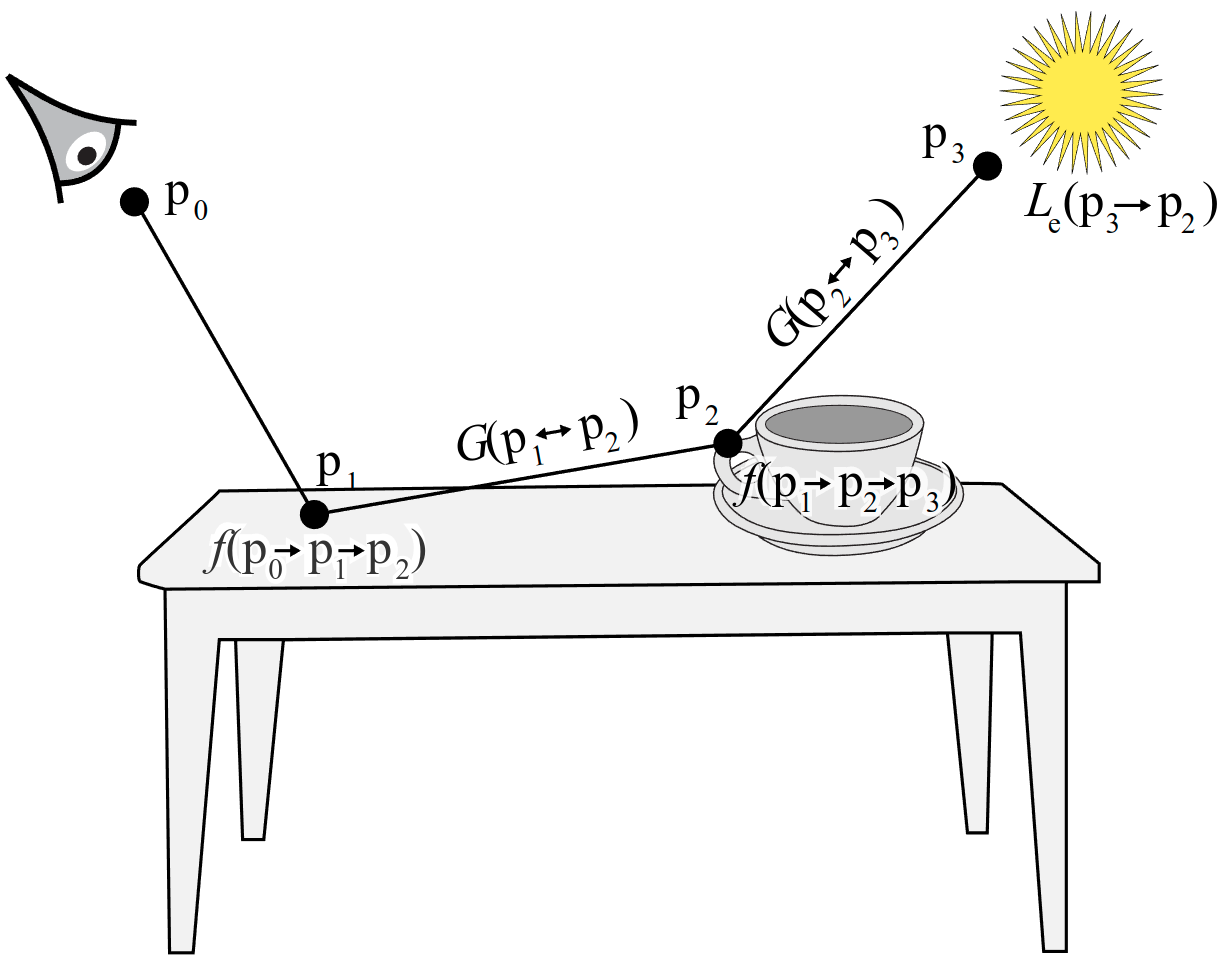
\includegraphics[width=0.8\linewidth]{../assets/chapter8_light_transport_equation.png}
	\caption{Illustrazione della Forma orientata su integrali di percorsi della rendering equation. Immagine da \cite{pharr}}
	\label{chapter8:LTE:pathFig}
\end{figure}
\section{Path Integral della Rendering Equation}
Abbiamo espresso, con Equazione \ref{chapter3:surface:areaRenderingEq}, la rendering equation in termini dell'unione di tutte le porzioni di 
superfici visibili dal punto $\vec{p}$, qui riportata
\begin{equation*}
	L(\vec{p},\hat{pq}) %
		= L_e(\vec{p},\hat{pq}) + \int_{A}f_s(\vec{p},\hat{\omega}_o,\hat{pq})G(\vec{p},\vec{q})L(\vec{q},-\hat{pq})\mathrm{d}A(\vec{q})
\end{equation*}
Si noti che un'equazione di questo tipo ha struttura nota come \textit{Equazione Integrale di Fredholm del secondo tipo}.\\
Definendo notazione \mbox{$L_{o|e}(\vec{p}_{i+1}\to\vec{p}_i)=L_{o|e}(\vec{p}_{i+1},\hat{p_ip_{i+1}})$} e \\
\mbox{$f_r(\vec{p}_i,\vec{p}_{i+1},\vec{p}_{i+2})=f_r(\vec{p}_{i+1},\hat{p_ip_{i+1}},\hat{p_{i+1},p_{i+2}})$}, posso riscrivere tale equazione nella 
\textit{three-point form}
\begin{equation}\label{chapter8:LTE:3pointform}
	L(\vec{p}_1\to\vec{p}_0) %
		= L_e(\vec{p}_1\to\vec{p}_0)+\int_{A}f_s(\vec{p}_0,\vec{p}_1,\vec{p}_2)G(\vec{p}_1,\vec{p}_2)L(\vec{p}_2\to\vec{p}_1)\mathrm{d}A(\vec{p}_2)
\end{equation}
Dove ricordiamo il termine geometrico che lega le varie superfici \`e dato da Equazione \ref{chapter3:surface:geometricTerm}. La differenza tra 
la Rendering Equation sulla sfera di direzioni e questa forma consiste nel fatto che per valutare la prima, campioneremmo da una distribuzione di 
direzioni per generare raggi e valutare la funzione integranda ricorsivamente. In questa forma, campioneremmo punti sulle superfici seguendo una 
distribuzione sulle aree, ne calcoleremmo il termine geometrico, e genereremmo raggi per valutare la funzione di visibilit\`a 
\mbox{$V(\vec{p}_i,\vec{p}_{i+1})$}.\par 
La forma pi\`u flessibile della Equazione \ref{chapter8:LTE:3pointform} consiste in una formulazione che esprime la radianza come un integrale su 
dei percorsi, rappresentati come punti in uno spazio con alta dimensionalit\`a (vedi Figura \ref{chapter8:LTE:pathFig}), il quale ci permette di 
stabilire strategie sulla scelta di paths da valutare per poter sviluppare algoritmi efficienti. Per poter esplicitare tale forma espandiamo la 
definizione ricorsiva di radianza, e raggruppiamo i termini per complessit\`a
\begin{align}
	L(\vec{p}_1\to\vec{p}_0)&=L_e(\vec{p}_1\to\vec{p}_0) \nonumber \\
		&+\int_{A}L_e(\vec{p}_2\to\vec{p}_1)f_s(\vec{p}_0,\vec{p}_1,\vec{p}_2)G(\vec{p}_1,\vec{p}_2)\mathrm{d}A(\vec{p}_2) \nonumber \\
		&+\int_{A}\int_{A}L_e(\vec{p}_3\to\vec{p}_2)f_s(\vec{p}_1,\vec{p}_2,\vec{p}_3)G(\vec{p}_2,\vec{p}_3)\mathrm{d}A(\vec{p}_3) \nonumber \\
		&+\ldots \nonumber \\
		&=\sum_{i=1}^\infty P(\bar{p}_n)
\end{align}
Dove $\bar{p}_n=\{\vec{p}_0,\vec{p}_1,\ldots,\vec{p}_n\}$.\par
$P(\bar{p}_n)$ restituisce la quantit\`a di radianza scattered lungo un percorso con 
gli $n+1$ vertici $\vec{p}_0,\vec{p}_1,\ldots,\vec{p}_n$, nei quali assumiamo $\vec{p}_0$ \`e sul film plane e $p_n$ \`e su una sorgente luminosa, 
pari a 
\begin{align}
	P(\bar{p}_n) &= \underbrace{\int_A\int_A\ldots\int_A}_{n-1\text{ volte}}L_e(\vec{p}_n\to\vec{p}_{n-1})\left(\prod_{i=1}^{n-1}%
		f_s(\vec{p}_{i-1},\vec{p}_i,\vec{p}_{i+1})G(\vec{p_{i+1},p_{i}})\right)\mathrm{d}A(\vec{p}_2)\ldots\mathrm{d}A(\vec{p}_n) \\
	P(\bar{p}_0) &= L_e(\vec{p}_1,\vec{p}_0) \nonumber
\end{align}
La produttoria evidenziata nell'n-esimo path integral \`e detta \textit{throughput} della path
\begin{equation}
	T(\bar{p}_n)=\prod_{i=1}^{n-1}f_s(\vec{p}_{i-1},\vec{p}_i,\vec{p}_{i+1})G(\vec{p_{i+1},p_{i}})
\end{equation}
Da cui 
\begin{equation}
	P(\bar{p}_n) = \underbrace{\int_A\int_A\ldots\int_A}_{n-1\text{ volte}}L_e(\vec{p}_n\to\vec{p}_{n-1})T(\bar{p}_n)%
		\mathrm{d}A(\vec{p}_2)\ldots\mathrm{d}A(\vec{p}_n)
\end{equation}
Notiamo che dei termini $P(\bar{p}_i)$ potrebbero contenere distribuzioni di Dirac all'interno della loro funzione integranda, dovuta o a determinati 
modelli di sorgenti luminose o BSDF. Dunque le implementazioni devono gestire tale caso particolare in quanto riduce la quantit\`a di termini della 
somma da stimare. Si consideri l'esempio da \cite{pharr} per l'illuminazione diretta con una sorgente puntiforme descritta da una distribuzione di 
Dirac.\par
Un approccio per partizionare la somma infinita di path integrals \`e la seguente:
\begin{equation}
	L(\vec{p}_1\to\vec{p}_0)=P(\bar{p}_1)+P(\bar{p}_2)+\sum_{i=3}^\infty P(\bar{p}_i)
\end{equation}
Dove il primo termine \`e calcolato facilmente valutando la radianza emessa dal punto $\vec{p}_1$ verso $\vec{p}_0$, il secondo integrale \`e stimato 
con accuratezza elevata e i restanti termini della somma sono stimati con un'approssimazione pi\`u grossolana. Inoltre, si potrebbero anche partizionare
gli integrali a seconda della categoria di sorgenti luminose e BSDF, ad esempio per distinguere sorgenti grandi da sorgenti piccole, e BSDF contenenti
$\delta(x)$ dal resto.
\section{Path Tracing}
Avendo ricavato una espressione facilmente manovrabile, siamo pronti a formulare un'algoritmo per la risoluzione dell'equazione di Rendering.\par
Chiaramente nella nostra computazione non abbiamo la possibilit\`a di valutare una serie, per cui applichiamo \textit{Russian Roulette} 
(\ref{chapter6:variance:russianRoulette}), valutando la terminazione della valutazione della serie ad ogni termine com probabilit\`a $q_i$, definite 
a priori. Un approccio per la scelta di tali probabilit\`a \`e la seguente (giustificata in \cite{pharr})
\begin{align}
	q_j&\sim\mathcal{U}\left(0,1-\max_{\lambda\in\Lambda}\left\{
		\eta\prod_{i=1}^{j-2}\frac{f_s(\vec{p}_{j-1},\vec{p}_j,\vec{p}_{j+1})}{p_\omega(\hat{\omega}_j)}\right\}\right)
\end{align}
dove $\hat{\omega}_j=(\vec{p}_{j+1}-\vec{p}_j)/\norm{\vec{p}_{j+1}-\vec{p}_j}$ e $p_\omega(\hat{\omega}_j)$ PDF della BSDF 
(\ref{chapter3:surface:brdf})\par
Applicando la compensazione per tale tecnica, lo stimatore unbiased diventa
\begin{equation}
	\frac{1}{1-q_1}\left(P(\bar{p}_1)+\frac{1}{1-q_2}\left(P(\bar{p}_2)+\frac{1}{1-q_3}\left(P(\bar{p}_3)+\ldots\right)\right)\right)
\end{equation}
In quanto il throughput totale della path
\begin{equation*}
	\beta=\prod_{i=1}^{j-2}\frac{f_s(\vec{p}_{j-1},\vec{p}_j,\vec{p}_{j+1})}{p_\omega(\hat{\omega}_j)}
\end{equation*}
decresce man mano che il tracing continua, \`e garantito che la valutazione della path termini in un tempo limitato. Si noti che nonostante Russian
Roulette aumenta l'MSE, in quanto si accumulano meno contributi, l'efficienza aumenta comunque per la notevole diminuzione del Running Time.\par
Per stimare ciascun path integral $P(\bar{p}_n)$, necessitiamo di $n+1$ vertici dei quali $\vec{p}_0$ sia sul film plane e $\vec{p}_n$ sia su una 
sorgente luminosa. Un approccio potrebbe essere campionare, dopo aver scelto il vertice sul film plane da cui partire, $n-2$ punti da tutte le 
superfici della scena con densit\`a di distribuzione uniforme, e l'ultimo campione su una delle superfici luminose presenti nella scena con equa
probabilit\`a. Tale approccio per\`o non conta la mutua visibilit\`a tra le superfici e pu\`o condurre a risultati con alta varianza, per via della 
presenza di paths con contributo nullo, e risultati incorretti, senza contare il fatto che tale metodo non supporta una gestione per le distribuzioni
contenenti il delta di Dirac. Una strategia valida \`e rappresentata invece dalla \textit{Costruzione Incrementale del percorso} \cite{pharr}:\par
partendo da un punto del film plane $\vec{p}_0$ (per il quale la direzione del raggio visivo \`e determinata geometricamente dal camera model),
si traccia un raggio per intersecare una superficie in $\vec{p}_1$. Da qui si ripete il procedimento descritto a seguire.\par
da $\vec{p}_i$ campiona una direzione dalla BSDF per ottenere una direzione $\hat{\omega}_i$ la quale, tracciato un raggio lungo essa, che conduce ad 
una nuova intersezione $\vec{p}_{i+1}$.\par
L'ultimo punto del path $\vec{p}_n$ deve terminare su una sorgente luminosa. L'approccio utilizzato per la determinazione della sorgente da utilizzare
\`e il Multiple Importance Sampling, utilizzando come densit\`a di distribuzione la PDF della BSDF dell'ultima superficie, $p_\omega$, e la PDF 
della sorgente luminosa selezionata per il calcolo della radianza uscente dall'ultima superficie, $p_l$. Si ricordi che tali PDF hanno come dominio
la sfera unitaria di possibili direzioni, ed 
in quanto il path integral \`e un integrale su un area, bisogna applicare la correzione (vedi Equazione \ref{chapter3:surface:areaRenderingEq})
\begin{equation}
	p_A(\vec{p}_i)=p_\omega(\hat{\omega}_{j-1})\frac{|\langle\hat{n},\hat{p}_i\rangle|}{\norm{\vec{p}_{i-1}-\vec{p}_i}^2}
\end{equation}
andandosi a semplificare con il termine geometrico\footnote{omesso l'Importance Sampling per semplicit\`a e per evidenziare i passaggi seguiti}
\begin{align}
	P(\bar{p}_n)&\approx L_e(\vec{p}_n\to\vec{p}_{n-1})\prod_{i=1}^{n-1}\frac{f_s(\vec{p}_{i-1},\vec{p}_i,\vec{p}_{i+1})G(\vec{p_{i+1},p_{i}})}
		{p_A(\vec{p}_{i+1})} \nonumber \\
	&=L_e(\vec{p}_n\to\vec{p}_{n-1})\prod_{i=1}^{n-1}\frac{f_s(\vec{p}_{i-1},\vec{p}_i,\vec{p}_{i+1})V(\vec{p}_{i+1},\vec{p}_i)
		\frac{|\cos\theta_{i+1}||\cos\theta_i|}{\norm{\vec{p}_{i+1}-\vec{p}_i}^2}}{p_A(\vec{p}_{i+1})} \nonumber \\
	&=L_e(\vec{p}_n\to\vec{p}_{n-1})\prod_{i=1}^{n-1}\frac{f_s(\vec{p}_{i-1},\vec{p}_i,\vec{p}_{i+1})V(\vec{p}_{i+1},\vec{p}_i)
		\frac{|\cos\theta_{i+1}||\cos\theta_i|}{\norm{\vec{p}_i-\vec{p}_{i+1}}^2}}
		{p_\omega(\omega_i)\frac{|\cos\theta_{i+1}|}{\norm{\vec{p}_i-\vec{p}_{i+1}}^2}} \nonumber \\
	&=L_e(\vec{p}_n\to\vec{p}_{n-1})\prod_{i=1}^{n-1}\frac{f_s(\vec{p}_{i-1},\vec{p}_i,\vec{p}_{i+1})V(\vec{p}_{i+1},\vec{p}_i)
		|\cos\theta_i|}{p_\omega(\omega_i)}
\end{align}
Dopodich\`e suddividiamo il termine di Direct Lighting applicando MIS
\begin{align}
	P(\bar{p}_i)&\approx w_l(\hat{\omega}_l)\frac{L_e(\vec{p}_l\to\vec{p}_{i-1})f_s(\vec{p}_{i-2},\vec{p}_{i-1},\vec{p}_l)
		|\cos\theta_l|V(\vec{p}_{i-1},\vec{p}_l)}{p_l(\hat{\omega}_l)}\beta \nonumber \\
	&+w_b(\hat{\omega}_e)\frac{L_e(\vec{p}_b\to\vec{p}_{i-1})f_s(\vec{p}_{i-2},\vec{p}_{i-1},\vec{p}_b)
		|\cos\theta_b|V(\vec{p}_{i-1},\vec{p}_b)}{p_b(\hat{\omega}_b)}\beta
\end{align}
dove i pesi sono calcolati con la \textit{balance heuristic} o la \textit{power heuristic} (Sezione \ref{chapter6:variance:importanceSampling}).\par
